% This template is borrowed from the Reed College LaTeX thesis template. Most of the work
% for the document class was done by Sam Noble (SN), as well as this
% template. Later comments etc. by Ben Salzberg (BTS). Additional
% restructuring and APA support by Jess Youngberg (JY).
% Your comments and suggestions are more than welcome; please email
% them to cus@reed.edu
%
% See http://web.reed.edu/cis/help/latex.html for help. There are a
% great bunch of help pages there, with notes on
% getting started, bibtex, etc. Go there and read it if you're not
% already familiar with LaTeX.
%
% Any line that starts with a percent symbol is a comment.
% They won't show up in the document, and are useful for notes
% to yourself and explaining commands.
% Commenting also removes a line from the document;
% very handy for troubleshooting problems. -BTS

% As far as I know, this follows the requirements laid out in
% the 2002-2003 Senior Handbook. Ask a librarian to check the
% document before binding. -SN

%%
%% Preamble
%%
% \documentclass{<something>} must begin each LaTeX document
\documentclass[12pt,twoside]{deuthesis}
% Packages are extensions to the basic LaTeX functions. Whatever you
% want to typeset, there is probably a package out there for it.
% Chemistry (chemtex), screenplays, you name it.
% Check out CTAN to see: http://www.ctan.org/
%%
\usepackage{graphicx,latexsym}
\usepackage{amsmath}
\usepackage{amssymb,amsthm}
\usepackage{longtable,booktabs,setspace}
\usepackage{chemarr} %% Useful for one reaction arrow, useless if you're not a chem major
\usepackage[hyphens]{url}
% Added by CII
\usepackage{hyperref}
\usepackage{lmodern}
\usepackage{float}
\floatplacement{figure}{H}
% End of CII addition
\usepackage{rotating}

% Next line commented out by CII
%%% \usepackage{natbib}
% Comment out the natbib line above and uncomment the following two lines to use the new
% biblatex-chicago style, for Chicago A. Also make some changes at the end where the
% bibliography is included.
%\usepackage{biblatex-chicago}
%\bibliography{thesis}


% Added by CII (Thanks, Hadley!)
% Use ref for internal links
\renewcommand{\hyperref}[2][???]{\autoref{#1}}
\def\chapterautorefname{Chapter}
\def\sectionautorefname{Section}
\def\subsectionautorefname{Subsection}
% End of CII addition

% Added by CII
\usepackage{caption}
\captionsetup{width=5in}
% End of CII addition

% \usepackage{times} % other fonts are available like times, bookman, charter, palatino

% Syntax highlighting #22
  \usepackage{color}
  \usepackage{fancyvrb}
  \newcommand{\VerbBar}{|}
  \newcommand{\VERB}{\Verb[commandchars=\\\{\}]}
  \DefineVerbatimEnvironment{Highlighting}{Verbatim}{commandchars=\\\{\}}
  % Add ',fontsize=\small' for more characters per line
  \usepackage{framed}
  \definecolor{shadecolor}{RGB}{248,248,248}
  \newenvironment{Shaded}{\begin{snugshade}}{\end{snugshade}}
  \newcommand{\AlertTok}[1]{\textcolor[rgb]{0.94,0.16,0.16}{#1}}
  \newcommand{\AnnotationTok}[1]{\textcolor[rgb]{0.56,0.35,0.01}{\textbf{\textit{#1}}}}
  \newcommand{\AttributeTok}[1]{\textcolor[rgb]{0.13,0.29,0.53}{#1}}
  \newcommand{\BaseNTok}[1]{\textcolor[rgb]{0.00,0.00,0.81}{#1}}
  \newcommand{\BuiltInTok}[1]{#1}
  \newcommand{\CharTok}[1]{\textcolor[rgb]{0.31,0.60,0.02}{#1}}
  \newcommand{\CommentTok}[1]{\textcolor[rgb]{0.56,0.35,0.01}{\textit{#1}}}
  \newcommand{\CommentVarTok}[1]{\textcolor[rgb]{0.56,0.35,0.01}{\textbf{\textit{#1}}}}
  \newcommand{\ConstantTok}[1]{\textcolor[rgb]{0.56,0.35,0.01}{#1}}
  \newcommand{\ControlFlowTok}[1]{\textcolor[rgb]{0.13,0.29,0.53}{\textbf{#1}}}
  \newcommand{\DataTypeTok}[1]{\textcolor[rgb]{0.13,0.29,0.53}{#1}}
  \newcommand{\DecValTok}[1]{\textcolor[rgb]{0.00,0.00,0.81}{#1}}
  \newcommand{\DocumentationTok}[1]{\textcolor[rgb]{0.56,0.35,0.01}{\textbf{\textit{#1}}}}
  \newcommand{\ErrorTok}[1]{\textcolor[rgb]{0.64,0.00,0.00}{\textbf{#1}}}
  \newcommand{\ExtensionTok}[1]{#1}
  \newcommand{\FloatTok}[1]{\textcolor[rgb]{0.00,0.00,0.81}{#1}}
  \newcommand{\FunctionTok}[1]{\textcolor[rgb]{0.13,0.29,0.53}{\textbf{#1}}}
  \newcommand{\ImportTok}[1]{#1}
  \newcommand{\InformationTok}[1]{\textcolor[rgb]{0.56,0.35,0.01}{\textbf{\textit{#1}}}}
  \newcommand{\KeywordTok}[1]{\textcolor[rgb]{0.13,0.29,0.53}{\textbf{#1}}}
  \newcommand{\NormalTok}[1]{#1}
  \newcommand{\OperatorTok}[1]{\textcolor[rgb]{0.81,0.36,0.00}{\textbf{#1}}}
  \newcommand{\OtherTok}[1]{\textcolor[rgb]{0.56,0.35,0.01}{#1}}
  \newcommand{\PreprocessorTok}[1]{\textcolor[rgb]{0.56,0.35,0.01}{\textit{#1}}}
  \newcommand{\RegionMarkerTok}[1]{#1}
  \newcommand{\SpecialCharTok}[1]{\textcolor[rgb]{0.81,0.36,0.00}{\textbf{#1}}}
  \newcommand{\SpecialStringTok}[1]{\textcolor[rgb]{0.31,0.60,0.02}{#1}}
  \newcommand{\StringTok}[1]{\textcolor[rgb]{0.31,0.60,0.02}{#1}}
  \newcommand{\VariableTok}[1]{\textcolor[rgb]{0.00,0.00,0.00}{#1}}
  \newcommand{\VerbatimStringTok}[1]{\textcolor[rgb]{0.31,0.60,0.02}{#1}}
  \newcommand{\WarningTok}[1]{\textcolor[rgb]{0.56,0.35,0.01}{\textbf{\textit{#1}}}}

% To pass between YAML and LaTeX the dollar signs are added by CII
\title{PROJE BAŞLIĞI}
%\author{Pelin PEKERMerve AKEdanur Binnaz DURSUNAhmet ÇALI} %Tek yazar için
\author{Pelin PEKER \\ Merve AK \\ Edanur Binnaz DURSUN \\ Ahmet ÇALI} %Çok yazar için
% The month and year that you submit your FINAL draft TO THE LIBRARY (May or December)
\date{Şubat 2024}
\division{İSTATİSTİK BÖLÜMÜ}
\advisor{Dr.~Engin YILDIZTEPE}
\institution{FEN FAKÜLTESİ}
\degree{Bitirme Projesi Raporu}
%If you have two advisors for some reason, you can use the following
% Uncommented out by CII
% End of CII addition

%%% Remember to use the correct department!
\department{İstatistik Bölümü}
% if you're writing a thesis in an interdisciplinary major,
% uncomment the line below and change the text as appropriate.
% check the Senior Handbook if unsure.
%\thedivisionof{The Established Interdisciplinary Committee for}
% if you want the approval page to say "Approved for the Committee",
% uncomment the next line
%\approvedforthe{Committee}

% Added by CII
%%% Copied from knitr
%% maxwidth is the original width if it's less than linewidth
%% otherwise use linewidth (to make sure the graphics do not exceed the margin)
\makeatletter
\def\maxwidth{ %
  \ifdim\Gin@nat@width>\linewidth
    \linewidth
  \else
    \Gin@nat@width
  \fi
}
\makeatother

\renewcommand{\contentsname}{Table of Contents}
% End of CII addition

\setlength{\parskip}{0pt}

% Added by CII

\providecommand{\tightlist}{%
  \setlength{\itemsep}{0pt}\setlength{\parskip}{0pt}}

\Acknowledgements{
Tüm çalışma süresince yönlendiriciliği, katkıları ve yardımları ile yanımızda olan danışmanımız Dr.~Engin YILDIZTEPE 'ye ve böyle bir çalışmayı yapmamız için bize fırsat tanıyan Dokuz Eylül Üniversitesi Fen Fakültesi İstatistik Bölümüne teşekkür ederiz.\\
\strut \\
\strut \\
Pelin PEKER\\
Merve AK\\
Edanur Binnaz DURSUN\\
Ahmet ÇALI\\
}

\Dedication{

}

\Preface{
``PROJE BAŞLIĞI'' başlıklı bitirme projesi raporu tarafımdan okunmuş, kapsamı ve niteliği açısından bir Bitirme Projesi raporu olarak kabul edilmiştir.\\
\strut \\
\strut \\
Dr.~Engin YILDIZTEPE
}

\AbstractTR{
Özet, çalışmanın önemini ve faydasını anlatan bir bölüm degildir. Çalısmayı ana
hatlarıyla anlatacak ve 300 kelimeyi aşmayacak şekilde hazırlanmalıdır. En az üç en
çok beş anahtar kelime ilgili yere yazılmalıdır.

\par

ikinci paragraf buradan başlar\\
\strut \\
\textbf{Anahtar Kelimeler:} anahtar kelime 1, anahtar kelime 2, anahtar kelime 3
}

\Abstract{
The preface pretty much says it all.

\par

Second paragraph of abstract starts here.\\
\strut \\
\textbf{Keywords:} keyword1, keyword2, keyword3
}


% End of CII addition
%%
%% End Preamble
%%
%
\begin{document}

% Everything below added by CII
  \maketitle

\frontmatter % this stuff will be roman-numbered
\pagestyle{empty} % this removes page numbers from the frontmatter
\begin{preface}
	``PROJE BAŞLIĞI'' başlıklı bitirme projesi raporu tarafımdan okunmuş, kapsamı ve niteliği açısından bir Bitirme Projesi raporu olarak kabul edilmiştir.\\
\strut \\
\strut \\
Dr.~Engin YILDIZTEPE
\end{preface}
  \begin{acknowledgements}
    Tüm çalışma süresince yönlendiriciliği, katkıları ve yardımları ile yanımızda olan danışmanımız Dr.~Engin YILDIZTEPE 'ye ve böyle bir çalışmayı yapmamız için bize fırsat tanıyan Dokuz Eylül Üniversitesi Fen Fakültesi İstatistik Bölümüne teşekkür ederiz.\\
    \strut \\
    \strut \\
    Pelin PEKER\\
    Merve AK\\
    Edanur Binnaz DURSUN\\
    Ahmet ÇALI\\
  \end{acknowledgements}
\begin{abstractTR}
	Özet, çalışmanın önemini ve faydasını anlatan bir bölüm degildir. Çalısmayı ana
hatlarıyla anlatacak ve 300 kelimeyi aşmayacak şekilde hazırlanmalıdır. En az üç en
çok beş anahtar kelime ilgili yere yazılmalıdır.

\par

ikinci paragraf buradan başlar\\
\strut \\
\textbf{Anahtar Kelimeler:} anahtar kelime 1, anahtar kelime 2, anahtar kelime 3
\end{abstractTR}
\begin{abstract}
	The preface pretty much says it all.

\par

Second paragraph of abstract starts here.\\
\strut \\
\textbf{Keywords:} keyword1, keyword2, keyword3
\end{abstract}

  \hypersetup{linkcolor=black}
  \setcounter{tocdepth}{2}
  \tableofcontents

  \listoftables

  \listoffigures


% This was added by EY
\newlength{\cslhangindent}
\setlength{\cslhangindent}{1.5em}
\newenvironment{CSLReferences}%
  {}%
  {\par}
\newenvironment{cslreferences}%
  {}%
  {\par}

\mainmatter % here the regular arabic numbering starts
\pagestyle{fancyplain} % turns page numbering back on

\hypertarget{introduction}{%
\chapter*{Introduction}\label{introduction}}
\addcontentsline{toc}{chapter}{Introduction}

Welcome to the \emph{R Markdown} thesis template. This template is based on (and in many places copied directly from) the Reed College LaTeX template, but hopefully it will provide a nicer interface for those that have never used TeX or LaTeX before. Using \emph{R Markdown} will also allow you to easily keep track of your analyses in \textbf{R} chunks of code, with the resulting plots and output included as well. The hope is this \emph{R Markdown} template gets you in the habit of doing reproducible research, which benefits you long-term as a researcher, but also will greatly help anyone that is trying to reproduce or build onto your results down the road.

Hopefully, you won't have much of a learning period to go through and you will reap the benefits of a nicely formatted thesis. The use of LaTeX in combination with \emph{Markdown} is more consistent than the output of a word processor, much less prone to corruption or crashing, and the resulting file is smaller than a Word file. While you may have never had problems using Word in the past, your thesis is likely going to be about twice as large and complex as anything you've written before, taxing Word's capabilities. After working with \emph{Markdown} and \textbf{R} together for a few weeks, we are confident this will be your reporting style of choice going forward.

\textbf{Why use it?}

\emph{R Markdown} creates a simple and straightforward way to interface with the beauty of LaTeX. Packages have been written in \textbf{R} to work directly with LaTeX to produce nicely formatting tables and paragraphs. In addition to creating a user friendly interface to LaTeX, \emph{R Markdown} also allows you to read in your data, to analyze it and to visualize it using \textbf{R} functions, and also to provide the documentation and commentary on the results of your project. Further, it allows for \textbf{R} results to be passed inline to the commentary of your results. You'll see more on this later.

\textbf{Who should use it?}

Anyone who needs to use data analysis, math, tables, a lot of figures, complex cross-references, or who just cares about the final appearance of their document should use \emph{R Markdown}. Of particular use should be anyone in the sciences, but the user-friendly nature of \emph{Markdown} and its ability to keep track of and easily include figures, automatically generate a table of contents, index, references, table of figures, etc. should make it of great benefit to nearly anyone writing a thesis project.

\hypertarget{rmd-basics}{%
\chapter{R Markdown Basics}\label{rmd-basics}}

Here is a brief introduction into using \emph{R Markdown}. \emph{Markdown} is a simple formatting syntax for authoring HTML, PDF, and MS Word documents. \emph{R Markdown} provides the flexibility of \emph{Markdown} with the implementation of \textbf{R} input and output. For more details on using \emph{R Markdown} see \url{http://rmarkdown.rstudio.com}.

Be careful with your spacing in \emph{Markdown} documents. While whitespace largely is ignored, it does at times give \emph{Markdown} signals as to how to proceed. As a habit, try to keep everything left aligned whenever possible, especially as you type a new paragraph. In other words, there is no need to indent basic text in the Rmd document (in fact, it might cause your text to do funny things if you do).

\hypertarget{lists}{%
\section{Lists}\label{lists}}

It's easy to create a list. It can be unordered like
\begin{itemize}
\tightlist
\item
  Item 1
\item
  Item 2
\end{itemize}
or it can be ordered like
\begin{enumerate}
\def\labelenumi{\arabic{enumi}.}
\tightlist
\item
  Item 1
\item
  Item 2
\end{enumerate}
Notice that I intentionally mislabeled Item 2 as number 4. \emph{Markdown} automatically figures this out! You can put any numbers in the list and it will create the list. Check it out below.

To create a sublist, just indent the values a bit (at least four spaces or a tab). (Here's one case where indentation is key!)
\begin{enumerate}
\def\labelenumi{\arabic{enumi}.}
\tightlist
\item
  Item 1
\item
  Item 2
\item
  Item 3
  \begin{itemize}
  \tightlist
  \item
    Item 3a
  \item
    Item 3b
  \end{itemize}
\end{enumerate}
\hypertarget{line-breaks}{%
\section{Line breaks}\label{line-breaks}}

Make sure to add white space between lines if you'd like to start a new paragraph. Look at what happens below in the outputted document if you don't:

Here is the first sentence. Here is another sentence. Here is the last sentence to end the paragraph.
This should be a new paragraph.

\emph{Now for the correct way:}

Here is the first sentence. Here is another sentence. Here is the last sentence to end the paragraph.

This should be a new paragraph.

\hypertarget{r-chunks}{%
\section{R chunks}\label{r-chunks}}

When you click the \textbf{Knit} button above a document will be generated that includes both content as well as the output of any embedded \textbf{R} code chunks within the document. You can embed an \textbf{R} code chunk like this (\texttt{cars} is a built-in \textbf{R} dataset):
\begin{Shaded}
\begin{Highlighting}[]
\FunctionTok{summary}\NormalTok{(cars)}
\end{Highlighting}
\end{Shaded}
\begin{verbatim}
     speed           dist       
 Min.   : 4.0   Min.   :  2.00  
 1st Qu.:12.0   1st Qu.: 26.00  
 Median :15.0   Median : 36.00  
 Mean   :15.4   Mean   : 42.98  
 3rd Qu.:19.0   3rd Qu.: 56.00  
 Max.   :25.0   Max.   :120.00  
\end{verbatim}
\hypertarget{inline-code}{%
\section{Inline code}\label{inline-code}}

If you'd like to put the results of your analysis directly into your discussion, add inline code like this:
\begin{quote}
The \texttt{cos} of \(2 \pi\) is 1.
\end{quote}
Another example would be the direct calculation of the standard deviation:
\begin{quote}
The standard deviation of \texttt{speed} in \texttt{cars} is 5.2876444.
\end{quote}
One last neat feature is the use of the \texttt{ifelse} conditional statement which can be used to output text depending on the result of an \textbf{R} calculation:
\begin{quote}
The standard deviation is less than 6.
\end{quote}
Note the use of \texttt{\textgreater{}} here, which signifies a quotation environment that will be indented.

As you see with \texttt{\$2\ \textbackslash{}pi\$} above, mathematics can be added by surrounding the mathematical text with dollar signs. More examples of this are in \protect\hyperlink{math-sci}{Mathematics and Science} if you uncomment the code in \protect\hyperlink{math}{Math}.

\hypertarget{including-plots}{%
\section{Including plots}\label{including-plots}}

You can also embed plots. For example, here is a way to use the base \textbf{R} graphics package to produce a plot using the built-in \texttt{pressure} dataset:

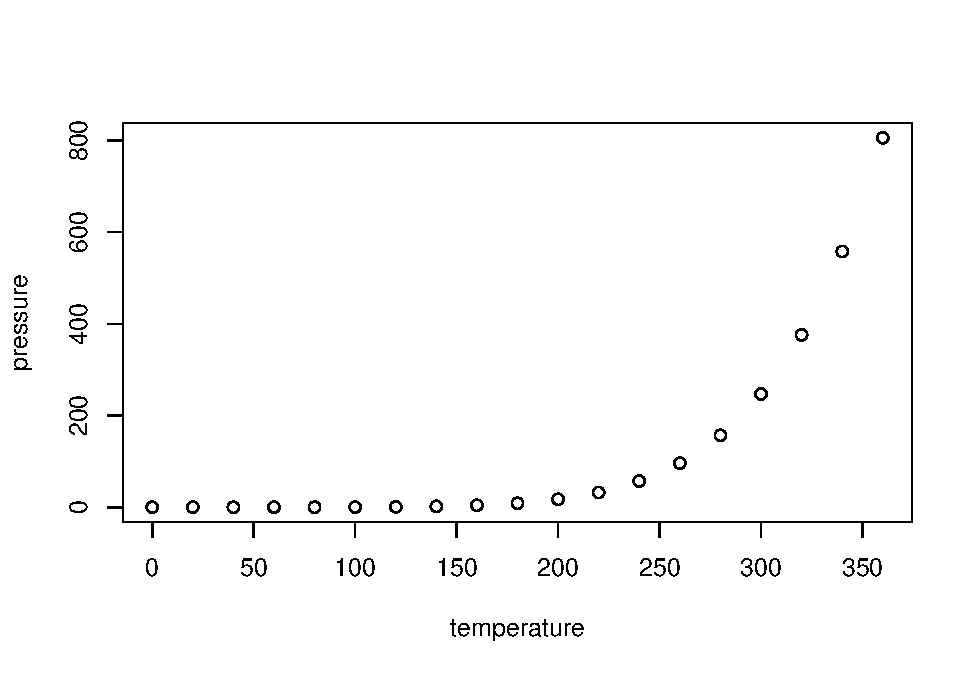
\includegraphics{BP_Rapor_files/figure-latex/pressure-1.pdf}

Note that the \texttt{echo=FALSE} parameter was added to the code chunk to prevent printing of the \textbf{R} code that generated the plot. There are plenty of other ways to add chunk options. More information is available at \url{http://yihui.name/knitr/options/}.

Another useful chunk option is the setting of \texttt{cache=TRUE} as you see here. If document rendering becomes time consuming due to long computations or plots that are expensive to generate you can use knitr caching to improve performance. Later in this file, you'll see a way to reference plots created in \textbf{R} or external figures.

\hypertarget{loading-and-exploring-data}{%
\section{Loading and exploring data}\label{loading-and-exploring-data}}

Included in this template is a file called \texttt{flights.csv}. This file includes a subset of the larger dataset of information about all flights that departed from Seattle and Portland in 2014. More information about this dataset and its \textbf{R} package is available at \url{http://github.com/ismayc/pnwflights14}. This subset includes only Portland flights and only rows that were complete with no missing values. Merges were also done with the \texttt{airports} and \texttt{airlines} data sets in the \texttt{pnwflights14} package to get more descriptive airport and airline names.

We can load in this data set using the following command:
\begin{Shaded}
\begin{Highlighting}[]
\NormalTok{flights }\OtherTok{\textless{}{-}} \FunctionTok{read.csv}\NormalTok{(}\StringTok{"data/flights.csv"}\NormalTok{)}
\end{Highlighting}
\end{Shaded}
The data is now stored in the data frame called \texttt{flights} in \textbf{R}. To get a better feel for the variables included in this dataset we can use a variety of functions. Here we can see the dimensions (rows by columns) and also the names of the columns.
\begin{Shaded}
\begin{Highlighting}[]
\FunctionTok{dim}\NormalTok{(flights)}
\end{Highlighting}
\end{Shaded}
\begin{verbatim}
[1] 52808    16
\end{verbatim}
\begin{Shaded}
\begin{Highlighting}[]
\FunctionTok{names}\NormalTok{(flights)}
\end{Highlighting}
\end{Shaded}
\begin{verbatim}
 [1] "month"        "day"          "dep_time"     "dep_delay"    "arr_time"    
 [6] "arr_delay"    "carrier"      "tailnum"      "flight"       "dest"        
[11] "air_time"     "distance"     "hour"         "minute"       "carrier_name"
[16] "dest_name"   
\end{verbatim}
Another good idea is to take a look at the dataset in table form. With this dataset having more than 50,000 rows, we won't explicitly show the results of the command here. I recommend you enter the command into the Console \textbf{\emph{after}} you have run the \textbf{R} chunks above to load the data into \textbf{R}.
\begin{Shaded}
\begin{Highlighting}[]
\FunctionTok{View}\NormalTok{(flights)}
\end{Highlighting}
\end{Shaded}
While not required, it is highly recommended you use the \texttt{dplyr} package to manipulate and summarize your data set as needed. It uses a syntax that is easy to understand using chaining operations. Below I've created a few examples of using \texttt{dplyr} to get information about the Portland flights in 2014. You will also see the use of the \texttt{ggplot2} package, which produces beautiful, high-quality academic visuals.

We begin by checking to ensure that needed packages are installed and then we load them into our current working environment:
\begin{Shaded}
\begin{Highlighting}[]
\CommentTok{\# List of packages required for this analysis}
\CommentTok{\#pkg \textless{}{-} c("dplyr", "ggplot2", "knitr", "bookdown", "remotes")}
\NormalTok{pkg }\OtherTok{\textless{}{-}} \FunctionTok{c}\NormalTok{(}\StringTok{"tidyverse"}\NormalTok{, }\StringTok{"knitr"}\NormalTok{, }\StringTok{"bookdown"}\NormalTok{, }\StringTok{"remotes"}\NormalTok{)}
\CommentTok{\# Check if packages are not installed and assign the}
\CommentTok{\# names of the packages not installed to the variable new.pkg}
\NormalTok{new.pkg }\OtherTok{\textless{}{-}}\NormalTok{ pkg[}\SpecialCharTok{!}\NormalTok{(pkg }\SpecialCharTok{\%in\%} \FunctionTok{installed.packages}\NormalTok{())]}
\CommentTok{\# If there are any packages in the list that aren\textquotesingle{}t installed,}
\CommentTok{\# install them}
\ControlFlowTok{if}\NormalTok{ (}\FunctionTok{length}\NormalTok{(new.pkg))}
  \FunctionTok{install.packages}\NormalTok{(new.pkg)}
\CommentTok{\# Load packages (thesisdown will load all of the packages as well)}
\FunctionTok{library}\NormalTok{(thesisdown)}
\CommentTok{\#library(dplyr)}
\CommentTok{\#library(ggplot2)}
\FunctionTok{library}\NormalTok{(tidyverse)}
\FunctionTok{library}\NormalTok{(bookdown)}
\FunctionTok{library}\NormalTok{(knitr)}
\end{Highlighting}
\end{Shaded}
\clearpage

The example we show here does the following:
\begin{itemize}
\item
  Selects only the \texttt{carrier\_name} and \texttt{arr\_delay} from the \texttt{flights} dataset and then assigns this subset to a new variable called \texttt{flights2}.
\item
  Using \texttt{flights2}, we determine the largest arrival delay for each of the carriers.
\end{itemize}
\begin{Shaded}
\begin{Highlighting}[]
\NormalTok{flights2 }\OtherTok{\textless{}{-}}\NormalTok{ flights }\SpecialCharTok{\%\textgreater{}\%} 
  \FunctionTok{select}\NormalTok{(carrier\_name, arr\_delay)}
\NormalTok{max\_delays }\OtherTok{\textless{}{-}}\NormalTok{ flights2 }\SpecialCharTok{\%\textgreater{}\%} 
  \FunctionTok{group\_by}\NormalTok{(carrier\_name) }\SpecialCharTok{\%\textgreater{}\%}
  \FunctionTok{summarize}\NormalTok{(}\AttributeTok{max\_arr\_delay =} \FunctionTok{max}\NormalTok{(arr\_delay, }\AttributeTok{na.rm =} \ConstantTok{TRUE}\NormalTok{))}
\end{Highlighting}
\end{Shaded}
A useful function in the \texttt{knitr} package for making nice tables in \emph{R Markdown} is called \texttt{kable}. It is much easier to use than manually entering values into a table by copying and pasting values into Excel or LaTeX. This again goes to show how nice reproducible documents can be! (Note the use of \texttt{results="asis"}, which will produce the table instead of the code to create the table.) The \texttt{caption.short} argument is used to include a shorter title to appear in the List of Tables.
\begin{Shaded}
\begin{Highlighting}[]
\FunctionTok{kable}\NormalTok{(max\_delays, }
      \AttributeTok{col.names =} \FunctionTok{c}\NormalTok{(}\StringTok{"Airline"}\NormalTok{, }\StringTok{"Max Arrival Delay"}\NormalTok{),}
      \AttributeTok{caption =} \StringTok{"Maximum Delays by Airline"}\NormalTok{,}
      \AttributeTok{caption.short =} \StringTok{"Max Delays by Airline"}\NormalTok{,}
      \AttributeTok{longtable =} \ConstantTok{TRUE}\NormalTok{,}
      \AttributeTok{booktabs =} \ConstantTok{TRUE}\NormalTok{)}
\end{Highlighting}
\end{Shaded}
\begin{longtable}[t]{lr}
\caption[Max Delays by Airline]{\label{tab:maxdelays}Maximum Delays by Airline}\\
\toprule
Airline & Max Arrival Delay\\
\midrule
Alaska Airlines Inc. & 338\\
American Airlines Inc. & 1539\\
Delta Air Lines Inc. & 651\\
Frontier Airlines Inc. & 575\\
Hawaiian Airlines Inc. & 407\\
\addlinespace
JetBlue Airways & 273\\
SkyWest Airlines Inc. & 421\\
Southwest Airlines Co. & 694\\
US Airways Inc. & 347\\
United Air Lines Inc. & 472\\
\addlinespace
Virgin America & 366\\
\bottomrule
\end{longtable}
The last two options make the table a little easier-to-read.

We can further look into the properties of the largest value here for American Airlines Inc.~To do so, we can isolate the row corresponding to the arrival delay of 1539 minutes for American in our original \texttt{flights} dataset.
\begin{Shaded}
\begin{Highlighting}[]
\NormalTok{flights }\SpecialCharTok{\%\textgreater{}\%} \FunctionTok{filter}\NormalTok{(arr\_delay }\SpecialCharTok{==} \DecValTok{1539}\NormalTok{, }
\NormalTok{                  carrier\_name }\SpecialCharTok{==} \StringTok{"American Airlines Inc."}\NormalTok{) }\SpecialCharTok{\%\textgreater{}\%}
  \FunctionTok{select}\NormalTok{(}\SpecialCharTok{{-}}\FunctionTok{c}\NormalTok{(month, day, carrier, dest\_name, hour, }
\NormalTok{            minute, carrier\_name, arr\_delay))}
\end{Highlighting}
\end{Shaded}
\begin{verbatim}
  dep_time dep_delay arr_time tailnum flight dest air_time distance
1     1403      1553     1934  N595AA   1568  DFW      182     1616
\end{verbatim}
We see that the flight occurred on March 3rd and departed a little after 2 PM on its way to Dallas/Fort Worth. Lastly, we show how we can visualize the arrival delay of all departing flights from Portland on March 3rd against time of departure.
\begin{Shaded}
\begin{Highlighting}[]
\NormalTok{flights }\SpecialCharTok{\%\textgreater{}\%} \FunctionTok{filter}\NormalTok{(month }\SpecialCharTok{==} \DecValTok{3}\NormalTok{, day }\SpecialCharTok{==} \DecValTok{3}\NormalTok{) }\SpecialCharTok{\%\textgreater{}\%}
  \FunctionTok{ggplot}\NormalTok{(}\FunctionTok{aes}\NormalTok{(}\AttributeTok{x =}\NormalTok{ dep\_time, }\AttributeTok{y =}\NormalTok{ arr\_delay)) }\SpecialCharTok{+} \FunctionTok{geom\_point}\NormalTok{()}
\end{Highlighting}
\end{Shaded}
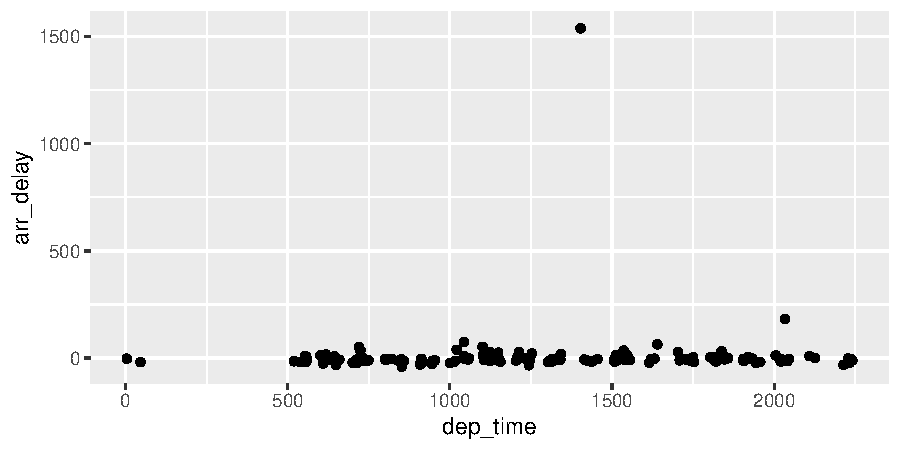
\includegraphics{BP_Rapor_files/figure-latex/march3plot-1.pdf}

\hypertarget{additional-resources}{%
\section{Additional resources}\label{additional-resources}}
\begin{itemize}
\item
  \emph{Markdown} Cheatsheet - \url{https://github.com/adam-p/markdown-here/wiki/Markdown-Cheatsheet}
\item
  \emph{R Markdown} Reference Guide - \url{https://www.rstudio.com/wp-content/uploads/2015/03/rmarkdown-reference.pdf}
\item
  Introduction to \texttt{dplyr} - \url{https://cran.rstudio.com/web/packages/dplyr/vignettes/introduction.html}
\item
  \texttt{ggplot2} Documentation - \url{http://docs.ggplot2.org/current/}
\end{itemize}
\hypertarget{math-sci}{%
\chapter{Mathematics and Science}\label{math-sci}}

\hypertarget{math}{%
\section{Math}\label{math}}

\TeX~is the best way to typeset mathematics. Donald Knuth designed \TeX~when he got frustrated at how long it was taking the typesetters to finish his book, which contained a lot of mathematics. One nice feature of \emph{R Markdown} is its ability to read LaTeX code directly.

If you are doing a thesis that will involve lots of math, you will want to read the following section which has been commented out. If you're not going to use math, skip over or delete this next commented section.

\hypertarget{uxe7oklu-deux11fiux15fim-noktasi}{%
\section{ÇOKLU DEĞİŞİM NOKTASI}\label{uxe7oklu-deux11fiux15fim-noktasi}}

Chemical formulas will look best if they are not italicized. Get around math mode's automatic italicizing in LaTeX by using the argument \texttt{\$\textbackslash{}mathrm\{formula\ here\}\$}, with your formula inside the curly brackets. (Notice the use of the backticks here which enclose text that acts as code.)

So, \(\mathrm{Fe_2^{2+}Cr_2O_4}\) is written \texttt{\$\textbackslash{}mathrm\{Fe\_2\^{}\{2+\}Cr\_2O\_4\}\$}.

\noindent Exponent or Superscript: \(\mathrm{O^-}\)

\noindent Subscript: \(\mathrm{CH_4}\)

To stack numbers or letters as in \(\mathrm{Fe_2^{2+}}\), the subscript is defined first, and then the superscript is defined.

\noindent Bullet: CuCl \(\bullet\) \(\mathrm{7H_{2}O}\)

\noindent Delta: \(\Delta\)

\noindent Reaction Arrows: \(\longrightarrow\) or \(\xrightarrow{solution}\)

\noindent Resonance Arrows: \(\leftrightarrow\)

\noindent Reversible Reaction Arrows: \(\rightleftharpoons\)

\hypertarget{ikili-segmentasyon-algoritmasux131}{%
\subsection{İkili Segmentasyon Algoritması}\label{ikili-segmentasyon-algoritmasux131}}

İkili segmentasyon algoritması (BinSeg), değişim noktası literatüründe kullanılan en köklü arama yöntemidir. İkili segmentasyon arama algoritmasının erken uygulamaları arasında Scott ve Knott (1974) ile Sen ve Srivastava (1975) bulunmaktadır.

İkili segmentasyon, herhangi bir tek değişim noktası yöntemini ardışık olarak farklı veri setlerinde tekrarlayarak çoklu değişim noktalarına genişletmek için kullanılabilir. İlk olarak, tek bir değişim noktası test istatistiğini tüm veri setine uygular. \(y_{1},y_{2},...,y_{n}\) şeklindeki veri seti üzerinde bir başlangıç noktası belirlenir. Bu başlangıç noktası, veri setinin ortalaması, medyanı veya başka bir özelliği olabilir. Belirlenen başlangıç noktasında bir değişim noktası testi yapılır. Bu test, veri setini iki alt küme olarak böldüğünde, oluşan alt kümelerin toplam maliyetinin belirli bir kritere göre düşük olup olmadığını kontrol eder, yani bir \(\tau\)'nin aşağıdaki koşulu sağlayıp sağlamadığını test eder:

\[C(y_{1:\tau}) + C(y_{(\tau+1):n}) + \beta < C(y_{1:n})\]

Burada:
\begin{itemize}
\item\textbf{C}:Bir segment için maliyet fonksiyonu
\item\textbf{$y_{1:\tau}$}:Başlangıçtan değişim noktasına kadar olan veri seti
\item\textbf{$y_{(\tau+1):n}$}:Değişim noktasından sona kadar olan veri seti
\item\textbf{$\beta$}:Aşırı uyum karşısında koruma sağlayan ceza terimi
\end{itemize}
Eğer bu koşul sağlanmıyorsa, o zaman herhangi bir değişim noktası tespit edilememiştir ve algoritma durur. Aksi takdirde veri, belirlenen değişim noktasından önce ve sonra olmak üzere iki segmente bölünür. Tek değişim noktası tespit yöntemi, değişiklikten önce ve sonra iki yeni segmente de tekrarlanır. Her iki segmentte de değişim noktaları belirlenirse, bunları yeni belirlenen değişim noktasında daha fazla segmentlere böler ve her yeni segmente değişim noktası tespit yöntemini uygular. Bu süreç, verinin herhangi bir bölümünde değişim noktası bulunamayana kadar devam eder.

Çoklu değişim noktalarını belirlemek için yaygın olarak kullanılan bir yaklaşım, aşağıdaki ifadeyi minimize etmektir:

\[\sum_{i=1}^{m+1} C(y(\tau_{i-1}+1):\tau_i) + \beta f(m)\]

Burada, \(C\) bir segment için bir maliyet fonksiyonu ve \(\beta f(m)\) aşırı uyum karşısında koruma sağlayan bir ceza terimidir.

İkili segmentasyon, herhangi bir değişim noktasının konumu önceden belirlenmiş değişim noktalarına bağlı olduğu için (\(f(m) = m\) olarak) yukarıdaki denklemin yaklaşık bir minimize edilmesidir. Algoritmanın her adımı, bu denklemi azaltıyorsa ek bir değişim noktası eklemeye çalışır. İkili segmentasyon algoritmasının avantajı, \(n\)'nin veri uzunluğu olduğu durumda \(O(n)\) hesaplama maliyeti ile uygulanabilen hızlı bir algoritma olmasıdır. Ancak, \(C\)'yi uygun bir şekilde seçmek zor olabilir ve farklı \(C\) seçimleri, değişim noktalarının sayısının tahmininde önemli farklara neden olabilir.

\hypertarget{pelt}{%
\subsection{PELT}\label{pelt}}

\hypertarget{paruxe7alux131-regresyon}{%
\subsection{Parçalı Regresyon}\label{paruxe7alux131-regresyon}}

Parçalı veya kesik çizgili modeller, yanıt ile bir veya daha fazla açıklayıcı değişken arasındaki ilişkilerin parçalı doğrusal olduğu, yani iki veya daha fazla değişkenle temsil edildiği regresyon modelleridir.Bu ilişkiler, genellikle bilinmeyen değerlerde birleştirilen iki veya daha fazla düz çizgi tarafından temsil edilir, bu değerlere genellikle kırılma noktaları, değişim noktaları veya birleşim noktaları denir. Bu yöntemde bağımsız değişken, aralıklara bölünür ve her bir aralığa ayrı bir çizgi segmenti uyarlanır.Parçalı regresyon analizi ayrıca çeşitli bağımsız değişkenlerle yapılan çok değişkenli veriler üzerinde de gerçekleştirilebilir. Parçalı regresyon analizi, bağımsız değişkenlerin belirli gruplara ayrıldığı durumlarda, bu gruplardaki değişkenler arasındaki ilişkilerin farklı olduğuna inanıldığında kullanışlıdır. Bu parçalar arasındaki sınırlar, değişim noktaları olarak adlandırılır.

Matematiksel olarak, model şu şekilde ifade edilebilir:

\(y = \beta_{0i} + \beta_{1i} x + \epsilon\)

Bu denklemde, \(\beta_{0i}\) ve \(\beta_{1i}\) sırasıyla i-inci segmentin kesişim noktası ve eğimini temsil eder.

Parçalı regresyon, ekonomi, biyoloji, çevre bilimleri, epidemiyoloji gibi çeşitli alanlarda kullanılır.Kalite iyileştirme müdahaleleriyle ilgili çalışmalarda parçalı regresyon analizlerinin kullanımına dair birçok örnek yayınlanmıştır.

Temel bir parçalı regresyon analizinde zaman periyodu müdahale öncesi ve sonrası parçalara bölünür ve her parçada ayrı ayrı kesişme noktaları ve eğimler tahmin edilir. Müdahaleden önce ve sonra kesişmelerde ve eğimlerdeki değişiklikleri test etmek için istatistiksel testler gerçekleştirilir. Veriler ve model spesifikasyonunda bazı basit değişikliklerle parçalı regresyon analizi, genellikle standart istatistiksel yazılım paketlerinde kolayca uygulanabilir. Genellikle, zaman içinde alınan gözlemler ilişkilidir, bu nedenle otokorelasyonu hesaba katmak için genellikle ek bir düzeltme yapılması gerekir.

Parçalı doğrusal regresyon, parçalı regresyonun doğrusal regresyon kullanılarak elde edilen bir alt türüdür.İki parçalı doğrusal regresyon, bir değişim noktası ile ayrılmış iki parçayla, değişken bir etkenin (x) yanıt fonksiyonunun (\(Y_{r}\)) ani bir değişikliğini nicelendirmek için kullanışlı olabilir. Değişim noktası, yanıt fonksiyonunun kritik, güvenli veya eşik değeri olarak yorumlanabilir; bu değerin ötesinde veya altında (istenmeyen) etkiler meydana gelebilir. Değişim noktası, karar verme süreçlerinde önemlidir.

Her bir parça için ayrı ayrı uygulanan en küçük kareler yöntemi, iki regresyon çizgisini veriye mümkün olduğunca iyi uyacak şekilde oluştururken, gözlemlenen (y) ve hesaplanan (Yr) bağımlı değişken değerleri arasındaki farkın karesini en aza indirir. Bu yöntemle şu iki denklem elde edilir:

\(Yr = A1.x+K1 <BP\) (değişim noktası için)

\(Yr = A2.x+K2 >BP\) (değişim noktası için)

Burada:
\begin{itemize}
\item $Y_{r}$, x'in belirli bir değeri için beklenen (tahmin edilen) y değeridir;
\item A1 ve A2 regresyon katsayılarıdır (çizgi segmentinin eğimini gösterir);
\item K1 ve K2 regresyon sabitleridir (y-ekseninde kesişimi gösterir).
\end{itemize}
Bu yöntem aynı zamanda iki korelasyon katsayısı (R) da üretir:

\(R_{1}^{2}=1-{\frac {\sum (y-Y_{r})^{2}}{\sum (y-Y_{a1})^{2}}}\) x\textless BP (değişim noktası için)

ve

\(R_{2}^{2}=1-{\frac {\sum (y-Y_{r})^{2}}{\sum (y-Y_{a2})^{2}}}\) x\textgreater BP (değişim noktası için)

Burada:
\begin{itemize}
\item $\sum (y-Y_{r})^{2}$  her bir parça için minimize edilmiş SSD'yi temsil eder
\item $Y_{a1}$ ve $Y_{a2}$ ilgili parçalarda y'nin ortalamasıdır.
\end{itemize}
En uygun eğilimi belirlemede, bu eğilimin güvenilir (anlamlı) olduğundan emin olmak için istatistiksel testler gerçekleştirilmelidir.

Eğer anlamlı bir değişim noktası tespit edilemezse, değişim noktası olmadan bir regresyona geçilmelidir.
Aşağıdaki istatistiksel testler, eğilim türünü belirlemek için kullanılır:
\begin{enumerate}
\item\textbf{A1 ve A2'nin Anlamlılığı:} A1 ve A2'nin anlamlılığı, A1 ve A2'nin standart hata SE'si ve Student'ün t-distribution'ı kullanılarak belirlenir.
\item\textbf{A1 ve A2'nin Farkının Anlamlılığı:} A1 ve A2'nin farkının anlamlılığı, farklarının standart hatası SE ve Student'ün t-distribution'ı kullanılarak belirlenir.
\item\textbf{Y1 ve Y2'nin Farkının Anlamlılığı:} Y1 ve Y2'nin farkının anlamlılığı, farklarının standart hatası SE ve Student'ün t-distribution'ı kullanılarak belirlenir.
\item\textbf{Değişim Noktasının Varlığını Test Etme:} Sözde skor testi, parçalı çizginin tahminini gerektirmez ve kırılma noktasının varlığını test etmek için daha formal bir istatistiksel yaklaşımdır.
\end{enumerate}
Ayrıca, tüm verilerin korelasyon katsayısı (\(R_{a}\)), belirleme katsayısı veya açıklama katsayısı, regresyon fonksiyonlarının güven aralıkları ve ANOVA analizi kullanılmaktadır.

\(C_{d}\) katsayısı, tüm veri seti için belirlenen şartlar altında maksimize edilmesi gereken bir belirleme katsayısıdır ve şu formülle hesaplanır:

\(C_{d}=1-{\sum (y-Y_{r})^{2} \over \sum (y-Y_{a})^{2}}\)

Burada \(Y_{r}\), önceki regresyon denklemlerine göre beklenen (tahmin edilen) y değeridir ve \(Y_{a}\), tüm y değerlerinin ortalamasıdır.

\(C_{d}\) katsayısı, 0 ile 1 arasında değer alır. Saf, parçalanmamış doğrusal regresyonda, \(C_{d}\) ve \(R_{a}^2\) değerleri eşittir. Parçalı regresyonda, \(C_{d}\)'nin \(R_{a}^2\)'den anlamlı derecede büyük olması, parçalanmanın haklı olduğunu gösterir.

Değişim noktasının en uygun değeri, \(C_{d}\) katsayısının maksimum olduğu noktada bulunabilir.

You may wish to put your reaction in an equation environment, which means that LaTeX will place the reaction where it fits and will number the equations for you.
\begin{equation}
  \mathrm{C_6H_{12}O_6  + 6O_2} \longrightarrow \mathrm{6CO_2 + 6H_2O}
  \label{eq:reaction}
\end{equation}
We can reference this combustion of glucose reaction via Equation \eqref{eq:reaction}.

\hypertarget{other-examples-of-reactions}{%
\subsection{Other examples of reactions}\label{other-examples-of-reactions}}

\(\mathrm{NH_4Cl_{(s)}}\) \(\rightleftharpoons\) \(\mathrm{NH_{3(g)}+HCl_{(g)}}\)

\noindent \(\mathrm{MeCH_2Br + Mg}\) \(\xrightarrow[below]{above}\) \(\mathrm{MeCH_2\bullet Mg \bullet Br}\)

\hypertarget{physics}{%
\section{Physics}\label{physics}}

Many of the symbols you will need can be found on the math page \url{http://web.reed.edu/cis/help/latex/math.html} and the Comprehensive LaTeX Symbol Guide (\url{http://mirror.utexas.edu/ctan/info/symbols/comprehensive/symbols-letter.pdf}).

\hypertarget{biology}{%
\section{Biology}\label{biology}}

You will probably find the resources at \url{http://www.lecb.ncifcrf.gov/~toms/latex.html} helpful, particularly the links to bsts for various journals. You may also be interested in TeXShade for nucleotide typesetting (\url{http://homepages.uni-tuebingen.de/beitz/txe.html}). Be sure to read the proceeding chapter on graphics and tables.

\hypertarget{ref-labels}{%
\chapter{Tables, Graphics, References, and Labels}\label{ref-labels}}

\hypertarget{tables}{%
\section{Tables}\label{tables}}

In addition to the tables that can be automatically generated from a data frame in \textbf{R} that you saw in \protect\hyperlink{rmd-basics}{R Markdown Basics} using the \texttt{kable} function, you can also create tables using \emph{pandoc}. (More information is available at \url{http://pandoc.org/README.html\#tables}.) This might be useful if you don't have values specifically stored in \textbf{R}, but you'd like to display them in table form. Below is an example. Pay careful attention to the alignment in the table and hyphens to create the rows and columns.

We can also create a link to the table by doing the following: Table \ref{tab:inher}. If you go back to \protect\hyperlink{loading-and-exploring-data}{Loading and exploring data} and look at the \texttt{kable} table, we can create a reference to this max delays table too: Table \ref{tab:maxdelays}. The addition of the \texttt{(\textbackslash{}\#tab:inher)} option to the end of the table caption allows us to then make a reference to Table \texttt{\textbackslash{}@ref(tab:label)}. Note that this reference could appear anywhere throughout the document after the table has appeared.

\clearpage

\hypertarget{figures}{%
\section{Figures}\label{figures}}

If your thesis has a lot of figures, \emph{R Markdown} might behave better for you than that other word processor. One perk is that it will automatically number the figures accordingly in each chapter. You'll also be able to create a label for each figure, add a caption, and then reference the figure in a way similar to what we saw with tables earlier. If you label your figures, you can move the figures around and \emph{R Markdown} will automatically adjust the numbering for you. No need for you to remember! So that you don't have to get too far into LaTeX to do this, a couple \textbf{R} functions have been created for you to assist. You'll see their use below.

In the \textbf{R} chunk below, we will load in a picture stored as \texttt{ist.png} in our ``figure'' directory. We then give it the caption of ``IST logo'', the label of ``istlogo'', and specify that this is a figure. Make note of the different \textbf{R} chunk options that are given in the R Markdown file (not shown in the knitted document).
\begin{Shaded}
\begin{Highlighting}[]
\FunctionTok{include\_graphics}\NormalTok{(}\AttributeTok{path =} \StringTok{"figure/ist.png"}\NormalTok{)}
\end{Highlighting}
\end{Shaded}
\begin{figure}

\includegraphics[width=4.44in]{figure/ist} \caption{IST logo}\label{fig:istlogo}
\end{figure}
Here is a reference to the IST logo: Figure \ref{fig:istlogo}. Note the use of the \texttt{fig:} code here. By naming the \textbf{R} chunk that contains the figure, we can then reference that figure later as done in the first sentence here. We can also specify the caption for the figure via the R chunk option \texttt{fig.cap}.

\clearpage

Below we will investigate how to save the output of an \textbf{R} plot and label it in a way similar to that done above. Recall the \texttt{flights} dataset from Chapter \ref{rmd-basics}. (Note that we've shown a different way to reference a section or chapter here.) We will next explore a bar graph with the mean flight departure delays by airline from Portland for 2014. Note also the use of the \texttt{scale} parameter which is discussed on the next page.
\begin{Shaded}
\begin{Highlighting}[]
\NormalTok{flights }\SpecialCharTok{\%\textgreater{}\%} \FunctionTok{group\_by}\NormalTok{(carrier) }\SpecialCharTok{\%\textgreater{}\%}
  \FunctionTok{summarize}\NormalTok{(}\AttributeTok{mean\_dep\_delay =} \FunctionTok{mean}\NormalTok{(dep\_delay)) }\SpecialCharTok{\%\textgreater{}\%}
  \FunctionTok{ggplot}\NormalTok{(}\FunctionTok{aes}\NormalTok{(}\AttributeTok{x =}\NormalTok{ carrier, }\AttributeTok{y =}\NormalTok{ mean\_dep\_delay)) }\SpecialCharTok{+}
  \FunctionTok{geom\_bar}\NormalTok{(}\AttributeTok{position =} \StringTok{"identity"}\NormalTok{, }\AttributeTok{stat =} \StringTok{"identity"}\NormalTok{, }\AttributeTok{fill =} \StringTok{"red"}\NormalTok{)}
\end{Highlighting}
\end{Shaded}
\begin{figure}
\centering
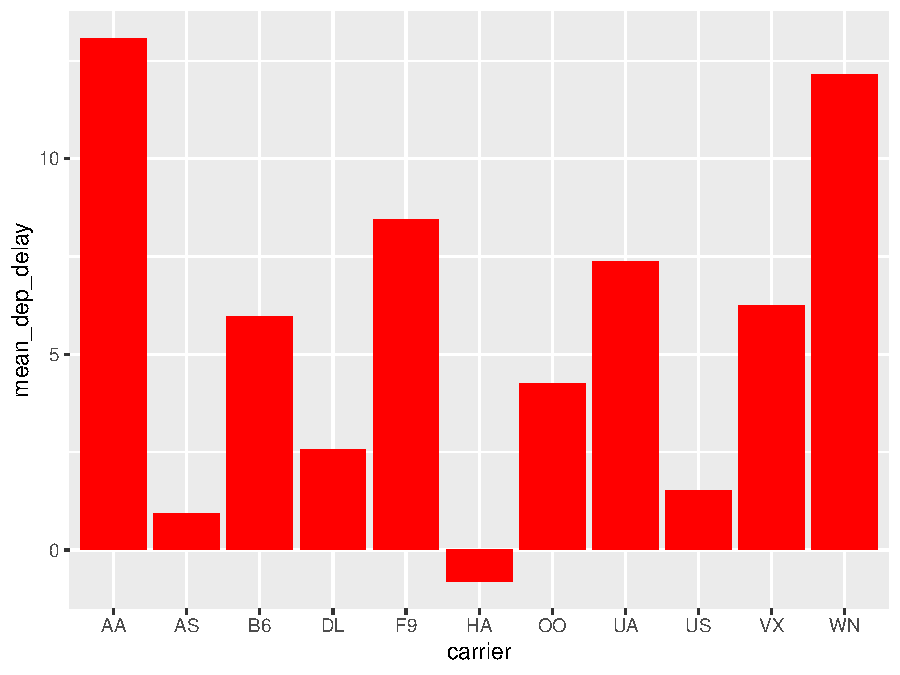
\includegraphics{BP_Rapor_files/figure-latex/delaysboxplot-1.pdf}
\caption{\label{fig:delaysboxplot}Mean Delays by Airline}
\end{figure}
Here is a reference to this image: Figure \ref{fig:delaysboxplot}.

A table linking these carrier codes to airline names is available at \url{https://github.com/ismayc/pnwflights14/blob/master/data/airlines.csv}.

\clearpage

Next, we will explore the use of the \texttt{out.extra} chunk option, which can be used to shrink or expand an image loaded from a file by specifying \texttt{"scale=\ "}. Here we use the mathematical graph stored in the ``subdivision.pdf'' file.
\begin{figure}
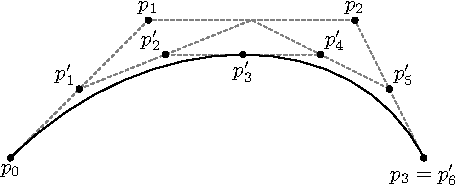
\includegraphics[scale=0.75]{figure/subdivision} \caption{Subdiv. graph}\label{fig:subd}
\end{figure}
Here is a reference to this image: Figure \ref{fig:subd}. Note that \texttt{echo=FALSE} is specified so that the \textbf{R} code is hidden in the document.

\textbf{More Figure Stuff}

Lastly, we will explore how to rotate and enlarge figures using the \texttt{out.extra} chunk option. (Currently this only works in the PDF version of the book.)
\begin{figure}
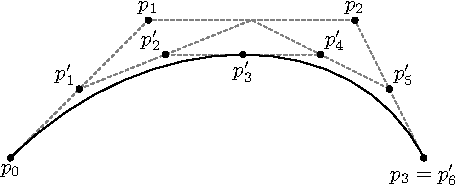
\includegraphics[angle=180, scale=1.1]{figure/subdivision} \caption{A Larger Figure, Flipped Upside Down}\label{fig:subd2}
\end{figure}
As another example, here is a reference: Figure \ref{fig:subd2}.

\hypertarget{footnotes-and-endnotes}{%
\section{Footnotes and Endnotes}\label{footnotes-and-endnotes}}

You might want to footnote something. \footnote{footnote text} The footnote will be in a smaller font and placed appropriately. Endnotes work in much the same way. More information can be found about both on the CUS site.

\hypertarget{bibliographies}{%
\section{Bibliographies}\label{bibliographies}}

Of course you will need to cite things, and you will probably accumulate an armful of sources. There are a variety of tools available for creating a bibliography database (stored with the .bib extension). In addition to BibTeX suggested below, you may want to consider using the free and easy-to-use tool called Zotero. The librarians have created Zotero documentation at \url{http://libguides.reed.edu/citation/zotero}. In addition, a tutorial is available from Middlebury College at \url{http://sites.middlebury.edu/zoteromiddlebury/}.

\emph{R Markdown} uses \emph{pandoc} (\url{http://pandoc.org/}) to build its bibliographies. One nice caveat of this is that you won't have to do a second compile to load in references as standard LaTeX requires. To cite references in your thesis (after creating your bibliography database), place the reference name inside square brackets and precede it by the ``at'' symbol. For example, here's a reference to a book about worrying: (Molina ve Borkovec, 1994). This \texttt{Molina1994} entry appears in a file called \texttt{thesis.bib} in the \texttt{bib} folder. This bibliography database file was created by a program called BibTeX. You can call this file something else if you like (look at the YAML header in the main .Rmd file) and, by default, is to placed in the \texttt{bib} folder.

For more information about BibTeX and bibliographies, see the CUS site \url{http://web.reed.edu/cis/help/latex/index.html}. There are three pages on this topic: \emph{bibtex} (which talks about using BibTeX, at \url{http://web.reed.edu/cis/help/latex/bibtex.html}), \emph{bibtexstyles} (about how to find and use the bibliography style that best suits your needs, at \url{http://web.reed.edu/cis/help/latex/bibtexstyles.html}) and \emph{bibman} (which covers how to make and maintain a bibliography by hand, without BibTeX, at \url{http://web.reed.edu/cis/help/latex/bibman.html}). The last page will not be useful unless you have only a few sources.

If you look at the YAML header at the top of the main .Rmd file you can see that we can specify the style of the bibliography by referencing the appropriate csl file. You can download a variety of different style files at \url{https://www.zotero.org/styles}. Make sure to download the file into the csl folder.

\textbf{Tips for Bibliographies}
\begin{itemize}
\tightlist
\item
  Like with thesis formatting, the sooner you start compiling your bibliography for something as large as thesis, the better. Typing in source after source is mind-numbing enough; do you really want to do it for hours on end in late April? Think of it as procrastination.
\item
  The cite key (a citation's label) needs to be unique from the other entries.
\item
  When you have more than one author or editor, you need to separate each author's name by the word ``and'' e.g.~\texttt{Author\ =\ \{Noble,\ Sam\ and\ Youngberg,\ Jessica\},}.
\item
  Bibliographies made using BibTeX (whether manually or using a manager) accept LaTeX markup, so you can italicize and add symbols as necessary.
\item
  To force capitalization in an article title or where all lowercase is generally used, bracket the capital letter in curly braces.
\item
  You can add a Thesis citation\footnote{Noble (2002)} option. The best way to do this is to use the phdthesis type of citation, and use the optional ``type'' field to enter ``Undergraduate thesis.''
\end{itemize}
\hypertarget{anything-else}{%
\section{Anything else?}\label{anything-else}}

If you'd like to see examples of other things in this template, please contact the \ldots. @ \ldots. team (email \href{mailto:email@email.email}{\nolinkurl{email@email.email}}) with your suggestions. We love to see people using \emph{R Markdown} for their theses, and are happy to help.

\hypertarget{Bolum4}{%
\chapter{Bölüm 4 Başlık}\label{Bolum4}}

\hypertarget{bu-bir-alt-baux15flux131k}{%
\section{Bu bir alt başlık}\label{bu-bir-alt-baux15flux131k}}

Bu bölümde şu konular yer almaktadır\ldots{}

\hypertarget{bu-ikinci-seviye-bir-alt-baux15flux131k}{%
\subsection{Bu ikinci seviye bir alt başlık}\label{bu-ikinci-seviye-bir-alt-baux15flux131k}}

\hypertarget{sonuuxe7}{%
\chapter*{Sonuç}\label{sonuuxe7}}
\addcontentsline{toc}{chapter}{Sonuç}

If we don't want Conclusion to have a chapter number next to it, we can add the \texttt{\{-\}} attribute.

\textbf{More info}

And here's some other random info: the first paragraph after a chapter title or section head \emph{shouldn't be} indented, because indents are to tell the reader that you're starting a new paragraph. Since that's obvious after a chapter or section title, proper typesetting doesn't add an indent there.

\hypertarget{kaynaklar}{%
\chapter*{Kaynaklar}\label{kaynaklar}}
\addcontentsline{toc}{chapter}{Kaynaklar}

\markboth{Kaynaklar}{Kaynaklar}

\hypertarget{refs}{}
\begin{CSLReferences}{1}{0}
\leavevmode\vadjust pre{\hypertarget{ref-angel2000}{}}%
Angel, E. (2000). \emph{Interactive Computer Graphics : A Top-Down Approach with OpenGL}. Boston, MA: Addison Wesley Longman.

\leavevmode\vadjust pre{\hypertarget{ref-angel2001a}{}}%
Angel, E. (2001a). \emph{Batch-file Computer Graphics : A Bottom-Up Approach with QuickTime}. Boston, MA: Wesley Addison Longman.

\leavevmode\vadjust pre{\hypertarget{ref-angel2001b}{}}%
Angel, E. (2001b). \emph{test second book by angel}. Boston, MA: Wesley Addison Longman.

\leavevmode\vadjust pre{\hypertarget{ref-deussen2000}{}}%
Deussen, O. ve Strothotte, T. (2000). Computer-Generated Pen-and-Ink Illustration of Trees. \emph{{``Proceedings of''} SIGGRAPH 2000}, Computer Graphics Proceedings, Annual Conference Series, 13-18.

\leavevmode\vadjust pre{\hypertarget{ref-hipr1997}{}}%
Fisher, R., Perkins, S., Walker, A. ve Wolfart, E. (1997). \emph{Hypermedia Image Processing Reference}. New York, NY: John Wiley \& Sons.

\leavevmode\vadjust pre{\hypertarget{ref-goochandgooch2001}{}}%
Gooch, B. ve Gooch, A. (2001a). \emph{{Non-Photorealistic Rendering}}. Natick, Massachusetts: A K Peters.

\leavevmode\vadjust pre{\hypertarget{ref-goochandgooch2001a}{}}%
Gooch, B. ve Gooch, A. (2001b). \emph{Test second book by gooches}. Natick, Massachusetts: A K Peters.

\leavevmode\vadjust pre{\hypertarget{ref-hertzmann2000}{}}%
Hertzmann, A. ve Zorin, D. (2000). Illustrating Smooth Surfaces. \emph{Proceedings of SIGGRAPH 2000}, Computer Graphics Proceedings, Annual Conference Series, \emph{5}(17), 517-526.

\leavevmode\vadjust pre{\hypertarget{ref-jain1989}{}}%
Jain, A. K. (1989). \emph{Fundamentals of Digital Image Processing}. Englewood Cliffs, New Jersey: Prentice-Hall.

\leavevmode\vadjust pre{\hypertarget{ref-Molina1994}{}}%
Molina, S. T. ve Borkovec, T. D. (1994). The {P}enn {S}tate Worry Questionnaire: Psychometric properties and associated characteristics. G. C. L. Davey ve F. Tallis (Ed.), \emph{Worrying: Perspectives on theory, assessment and treatment} içinde (ss. 265-283). New York: Wiley.

\leavevmode\vadjust pre{\hypertarget{ref-noble2002}{}}%
Noble, S. G. (2002). \emph{Turning images into simple line-art}. (Yayımlanmamış undergraduate thesis). Reed College.

\leavevmode\vadjust pre{\hypertarget{ref-reedweb2007}{}}%
Reed~College. (2007). LaTeX Your Document. \url{http://web.reed.edu/cis/help/LaTeX/index.html} adresinden erişildi.

\leavevmode\vadjust pre{\hypertarget{ref-russ1995}{}}%
Russ, J. C. (1995). \emph{{The Image Processing Handbook, Second Edition}}. Boca Raton, Florida: CRC Press.

\leavevmode\vadjust pre{\hypertarget{ref-salisbury1997}{}}%
Salisbury, M. P., Wong, M. T., Hughes, J. F. ve Salesin, D. H. (1997). Orientable Textures for Image-Based Pen-and-Ink Illustration. \emph{{``Proceedings of''} SIGGRAPH 97}, Computer Graphics Proceedings, Annual Conference Series, 401-406.

\leavevmode\vadjust pre{\hypertarget{ref-savitch2001}{}}%
Savitch, W. (2001). \emph{JAVA: An Introduction to Computer Science \& Programming}. Upper Saddle River, New Jersey: Prentice Hall.

\leavevmode\vadjust pre{\hypertarget{ref-tukey1984}{}}%
Tukey, J. W. (1984). \emph{The collected works of John W. Tukey} (C. 1). Taylor \& Francis.

\leavevmode\vadjust pre{\hypertarget{ref-wong1999}{}}%
Wong, E. (1999). \emph{{Artistic Rendering of Portrait Photographs}}. (Yayımlanmamış mathesis). Cornell University.

\end{CSLReferences}
\setlength{\parindent}{-0.20in}
\setlength{\leftskip}{0.20in}
\setlength{\parskip}{8pt}

\appendix

\hypertarget{ilk-ek-baux15flux131ux11fux131}{%
\chapter{İlk Ek Başlığı}\label{ilk-ek-baux15flux131ux11fux131}}

This first appendix includes all of the R chunks of code that were hidden throughout the document (using the \texttt{include\ =\ FALSE} chunk tag) to help with readibility and/or setup.

\textbf{In the main Rmd file}
\begin{Shaded}
\begin{Highlighting}[]
\CommentTok{\# This chunk ensures that the thesisdown package is}
\CommentTok{\# installed and loaded. This thesisdown package includes}
\CommentTok{\# the template files for the thesis.}
 \ControlFlowTok{if}\NormalTok{(}\SpecialCharTok{!}\FunctionTok{require}\NormalTok{(remotes)) }\FunctionTok{install.packages}\NormalTok{(}\StringTok{"remotes"}\NormalTok{, }\AttributeTok{repos =} \StringTok{"http://cran.rstudio.com"}\NormalTok{)}
 \ControlFlowTok{if}\NormalTok{(}\SpecialCharTok{!}\FunctionTok{require}\NormalTok{(thesisdown))remotes}\SpecialCharTok{::}\FunctionTok{install\_github}\NormalTok{(}\StringTok{"ismayc/thesisdown"}\NormalTok{)}
 \FunctionTok{library}\NormalTok{(thesisdown)}
\end{Highlighting}
\end{Shaded}
\textbf{In Chapter \ref{ref-labels}:}
\begin{Shaded}
\begin{Highlighting}[]
\CommentTok{\# This chunk ensures that the thesisdown package is}
\CommentTok{\# installed and loaded. This thesisdown package includes}
\CommentTok{\# the template files for the thesis and also two functions}
\CommentTok{\# used for labeling and referencing}
\ControlFlowTok{if}\NormalTok{(}\SpecialCharTok{!}\FunctionTok{require}\NormalTok{(remotes))}
  \FunctionTok{install.packages}\NormalTok{(}\StringTok{"remotes"}\NormalTok{, }\AttributeTok{repos =} \StringTok{"http://cran.rstudio.com"}\NormalTok{)}
\ControlFlowTok{if}\NormalTok{(}\SpecialCharTok{!}\FunctionTok{require}\NormalTok{(dplyr))}
    \FunctionTok{install.packages}\NormalTok{(}\StringTok{"dplyr"}\NormalTok{, }\AttributeTok{repos =} \StringTok{"http://cran.rstudio.com"}\NormalTok{)}
\ControlFlowTok{if}\NormalTok{(}\SpecialCharTok{!}\FunctionTok{require}\NormalTok{(ggplot2))}
    \FunctionTok{install.packages}\NormalTok{(}\StringTok{"ggplot2"}\NormalTok{, }\AttributeTok{repos =} \StringTok{"http://cran.rstudio.com"}\NormalTok{)}
\ControlFlowTok{if}\NormalTok{(}\SpecialCharTok{!}\FunctionTok{require}\NormalTok{(ggplot2))}
    \FunctionTok{install.packages}\NormalTok{(}\StringTok{"bookdown"}\NormalTok{, }\AttributeTok{repos =} \StringTok{"http://cran.rstudio.com"}\NormalTok{)}
\ControlFlowTok{if}\NormalTok{(}\SpecialCharTok{!}\FunctionTok{require}\NormalTok{(thesisdown))\{}
  \FunctionTok{library}\NormalTok{(remotes)}
\NormalTok{  remotes}\SpecialCharTok{::}\FunctionTok{install\_github}\NormalTok{(}\StringTok{"ismayc/thesisdown"}\NormalTok{)}
\NormalTok{  \}}
\FunctionTok{library}\NormalTok{(thesisdown)}
\NormalTok{flights }\OtherTok{\textless{}{-}} \FunctionTok{read.csv}\NormalTok{(}\StringTok{"data/flights.csv"}\NormalTok{)}
\end{Highlighting}
\end{Shaded}
\hypertarget{ikinci-ek-baux15flux131ux11fux131}{%
\chapter{İkinci Ek Başlığı}\label{ikinci-ek-baux15flux131ux11fux131}}

İkinci Ek




\end{document}
